\documentclass{amsart}
\usepackage{geometry}

\usepackage{amsmath, amssymb, latexsym}
\usepackage{tikz}
\usepackage{tikz-cd}
\usepackage{pgflibraryarrows}
\usepackage{pgflibrarysnakes}
\usepackage{color}

\usepackage[draft]{say}
\newcommand{\sayER}[1]{\say[ER]{\color{blue}{\bf ER:}\;#1}}
\newcommand{\sayDR}[1]{\say[DR]{\color{red}{\bf DR:}\;#1}}

\newtheorem{theorem}{Theorem}
\newtheorem{corollary}[theorem]{Corollary}
\newtheorem{example}[theorem]{Example}
\newtheorem{lemma}[theorem]{Lemma}
\newtheorem{remark}[theorem]{Remark}
\newtheorem{question}{Question}

\numberwithin{equation}{section}

\renewcommand{\AA}{\mathbb{A}}
\newcommand{\CC}{\mathbb{C}}
\newcommand{\PP}{\mathbb{P}}
\newcommand{\ZZ}{\mathbb{Z}}

\newcommand{\bfe}{\mathbf{e}}
\newcommand{\bff}{\mathbf{f}}
\newcommand{\bfg}{\mathbf{g}}
\newcommand{\bfu}{\mathbf{u}}

\newcommand{\cC}{\mathcal{C}}

\newcommand{\Hom}{\operatorname{Hom}}
\newcommand{\Span}{\operatorname{span}}

\newcommand{\udim}{\underline{\dim}\,}
\newcommand{\into}{\hookrightarrow}

\title{2-Kronecker Quiver Grassmannians}
\author{Ed Richmond}
\author{Dylan Rupel}

\begin{document}
  \maketitle

  \sayDR{This is a nice utility for commenting.}
  
   \sayER{Testing testing.} 

\section{Introduction}
  Quiver Grassmannians are projective varieties parametrizing subrepresentations of a given quiver representation.
  This provides a direct generalization of the standard Grassmannians of linear subspaces in which the geometry behind linear transformations is taken into account.
  Our goal in this project is to begin making explicit the geometry of the quiver Grassmannians.
  Unfortunately, in such an endeavor, it would be hopeless to expect a uniform description since every projective variety can be realized as an appropriate quiver Grassmannian \cite{reineke}.

  We therefore restrict in this note to the well-studied example of the \emph{Kronecker quiver} with two vertices and two parallel arrows as an initial proof of concept.
  In a subsequent work, we will utilize the results of \cite{rupel-weist} to extend our approach here to the Grassmannians of subrepresentations for the directly generalized $n$-Kronecker quivers (with an arbitrary number $n$ of parallel arrows between the pair of vertices); this simple case is already rich enough to encode the geometry of arbitrary projective varieties \sayDR{ToDo: Add a reference to Ringel} and so we restrict there and here to the ``rigid'' representations which offer a more uniform geometric structure.

  In the 2-Kronecker case, we focus on the case of indecomposable representations, though with the help of Caldero-Chapoton fibrations (c.f. Section~\ref{???}), this restriction is easily removed.
  These quiver Grassmannians have been extensively studied, in the process of constructing our main results we reproduce the cell decompositions obtained by Cerulli Irelli and Esposito \cite{cerulli irelli-esposito} in coordinates.
  This is the main tool allowing to deduce an explicit description of the closures of these affine cells.
  Unfortunately, this also demonstrates that this cellular decomposition does not provide the quiver Grassmannians with the structure of a CW-complex.
  However, the strange degenerations appear to be governed according to isomorphism type of the subrepresentations within the cells.

  Our approach builds from the explicit description of Pl\"ucker relations for quiver Grassmannians developed by Lorscheid and Weist \cite{lorscheid-weist} which we utilize to give an explicit parametrization of the affine cells in such cell decompositions.
  This provides the essential tool we will use for understanding cell closures.

\section{Standard Grassmannians}

  The quiver Grassmannians will be parametrized with respect to a particular choice of basis.
  Therefore, we will present the geometry of standard Grassmannians with respect to an explicit basis of the vector space.

  \subsection{Pl\"ucker Embedding}
  The \emph{Grassmannian} $Gr_e(\CC^n)$ is the projective variety of $e$-dimensional subspaces of $\CC^n$.
  Given a subspace $E \in Gr_e(\CC^n)$, a choice of basis for $E$ determines an $e\times n$ matrix $M(E)$.
  For $I \subset_e [n]$, we then get the value of the \emph{Pl\"ucker coordinate} $\Delta_I$ at the point $E$ as the $e\times e$ minor of $M(E)$ with columns labeled by $I$.
  As the Pl\"ucker coordinates depends on the choice of basis for $E$, they are only defined up to rescaling, i.e. the map
  \[E \mapsto [:\Delta_I:]_{I\subset_e[n]}\]
  defines an embedding $Gr_e(\CC^n)\into \PP^{{n \choose e} - 1}$.
  The image of this embedding is the closed subvariety defined by the \emph{Pl\"ucker relations}:
  \begin{equation}
    \label{eq:plucker}
    \sum_{i\in I'\setminus I} (-1)^{\epsilon(i,I)} \Delta_{I\cup\{i\}} \Delta_{I'\setminus\{i\}}=0
  \end{equation}
  for subsets $I \subset_{e-1} [n]$ and $I' \subset_{e+1} [n]$, where $\epsilon(i,I)=\#\{i'\in I:i'\le i\}$.

  \subsection{Pl\"ucker Coordinate Parametrization of Standard Schubert Cells}
  Consider a weight function $d:[n] \to \ZZ$ with $d(i)>d(j)$ for $i<j$.
  This gives rise to a $\CC^*$-action on $\CC^n$ given by $z.\bfu_i=z^{d(i)} \bfu_i$ for each standard basis vector $\bfu_i$. 
  In turn, we have an induced $\CC^*$-action on $Gr_e(\CC^n)$.
  The standard Schubert cells of $Gr_e(\CC^n)$ can be seen as the Bia\l{}ynicki-Birula attractor cells \cite{bb} for this action.

  More precisely, for $I \subset_e [n]$, write $E_I$ for the coordinate subspace $\langle \bfu_i \rangle_{i \in I}$.
  Then the \emph{Schubert cell} $\AA_I$ is given by
  \[\AA_I:=\{E\in Gr_e(\CC^n):\lim_{z\to0} z.E=E_I\}.\]
  \begin{lemma}
    The Schubert cell $\AA_I$ can be parametrized as an affine space by the normalized Pl\"ucker coordinates $\Delta_{I'}/\Delta_I$ for $I' \subset_e [n]$ with $|I\cap I'|=n-1$ and, writing $I\setminus I'=\{i\}$ and $I'\setminus I=\{j\}$, with $j<i$.
  \end{lemma}
  
  \begin{lemma}
    Let $V$ be a vector space and $W\subset V$ a subspace.
    There is a choice of basis of $V$ for which the closed embedding $Gr_e(W)\subset Gr_e(V)$ identifies $Gr_e(W)$ with a union of Schubert cells inside $Gr_e(V)$.
  \end{lemma}
  As a result, we will abuse notation slightly and remain ambiguous about the superset for a collection of indices $I$ labeling a Schubert cell $\AA_I$.

\section{Representations of the 2-Kronecker Quiver}

  Let $Q=1\substack{\longleftarrow\\\longleftarrow} 2$ be the \emph{2-Kronecker quiver} with arrows $Q_1=\{\alpha,\beta\}$.
  Write $W=\langle\alpha,\beta\rangle$ for the free group generated by the arrows of $Q$.
  There is a natural involution $\varphi$ of $W$ which interchanges the generators $\alpha$ and $\beta$.

  The \emph{universal covering quiver} $\widetilde Q$ of $Q$ is the quiver with vertex set $\widetilde Q_0=\{(i,w):i=1,2,\ w\in W\}$ and arrows $(\alpha,w):(2,w)\to(1,\alpha w)$ and $(\beta,w):(2,w)\to(1,\beta w)$ for $w\in W$.
  The automorphism $\varphi$ can be seen to act on $\widetilde Q_0$ via $\varphi\big((i,w)\big)=\big(i,\varphi(w)\big)$ for $i=1,2$ and on the arrows of $\widetilde Q$ via
  \[\varphi\big((\alpha,w)\big)=\big(\beta,\varphi(w)\big) \qquad \text{and} \qquad \varphi\big((\beta,w)\big)=\big(\alpha,\varphi(w)\big).\]
  We will only be interested in the two connected components of $\widetilde Q$ which are invariant under $\varphi$, namely those containing the vertices $(1,e)$ and $(2,e)$, where $e\in W$ is the identity element; these have the following forms:
  \[
    \begin{tikzcd}
      \widetilde Q^{(1)} := & \cdots & (1,\alpha\beta^{-1}) & & \fbox{$(1,e)$} & & (1,\beta\alpha^{-1}) & \cdots \\
      & \cdots \arrow["\beta"]{ur} & & (2,\beta^{-1}) \arrow["\alpha"']{ul} \arrow["\beta"]{ur} & & (2,\alpha^{-1}) \arrow["\alpha"']{ul} \arrow["\beta"]{ur} & & \cdots \arrow["\alpha"']{ul}
    \end{tikzcd}
  \]
  \[
    \begin{tikzcd}
      \hspace{-0.37cm} \widetilde Q^{(2)} := \hspace{0.37cm} & \cdots & & (1,\alpha) & & (1,\beta) & & \cdots \\
      & \cdots & (2,\beta^{-1}\alpha) \arrow["\alpha"']{ul} \arrow["\beta"]{ur} & & \fbox{$(2,e)$} \arrow["\alpha"']{ul} \arrow["\beta"]{ur} & & (2,\alpha^{-1}\beta) \arrow["\alpha"']{ul} \arrow["\beta"]{ur} & \cdots
    \end{tikzcd}
  \]
  The automorphism $\varphi$ then naturally acts on the categories of representations of $\widetilde Q^{(i)}$ for $i=1,2$.

  A \emph{representation} $M$ of $Q$ consists of a pair of vector spaces $M_1,M_2$ together with a pair of linear maps $M_\alpha,M_\beta:M_2\to M_1$.
  The \emph{dimension vector} of such a representation $M$ is the tuple $\udim M:=(\dim M_1,\dim M_2)$.

  We focus here on the indecomposable \emph{preprojective} representations $P_m$ of $Q$ having the dimension vector $(m,m-1)$ for $m\ge1$.
  These admit several natural lifts to $\widetilde Q$ which will be useful.
  The first, denoted $\widetilde P_m$, are invariant under $\varphi$ and have the following forms with $m$ copies of $\CC$ in the top row:
  \[
    \text{m odd: }
    \begin{tikzcd}
      \cdots & & \CC & \cdots & & \fbox{$\CC$} & & \cdots & \CC & & \cdots \\
      \cdots & 0 \arrow["\alpha"']{ul} \arrow["\beta"]{ur} & & \cdots \arrow["\alpha"']{ul} & \CC \arrow["\alpha"']{ul} \arrow["\beta"]{ur} & & \CC \arrow["\alpha"']{ul} \arrow["\beta"]{ur} & \cdots \arrow["\beta"]{ur} & & 0 \arrow["\alpha"']{ul} \arrow["\beta"]{ur} & \cdots
    \end{tikzcd}
  \]
  \[
    \text{m even: }
    \begin{tikzcd}
      \cdots & & \CC & \cdots & \CC & & \CC & \cdots & \CC & & \cdots \\
      \cdots & 0 \arrow["\alpha"']{ul} \arrow["\beta"]{ur} & & \cdots \arrow["\alpha"']{ul} \arrow["\beta"]{ur} & & \fbox{$\CC$} \arrow["\alpha"']{ul} \arrow["\beta"]{ur} & & \cdots \arrow["\alpha"']{ul} \arrow["\beta"]{ur} & & 0 \arrow["\alpha"']{ul} \arrow["\beta"]{ur} & \cdots
    \end{tikzcd}
  \]
  where:
  \begin{itemize}
    \item for $m$ odd, $P_m$ lifts to a representation $\widetilde P_m$ supported on $\widetilde Q^{(1)}$;
    \item for $m$ even, $P_m$ lifts to a representation $\widetilde P_m$ supported on $\widetilde Q^{(2)}$.
  \end{itemize}

  These choices of lift to $\widetilde Q$ induces a basis $\{v_{m,1},\cdots,v_{m,2m-1}\}$ of $P_m$ such that, for $t$ even, 
  \[\alpha(v_{m,t})=v_{m,t-1} \qquad \text{and} \qquad \beta(v_{m,t})=v_{m,t+1},\]
  i.e.\ we have the identifications
  \[P_{m,1}=\CC^m=\Span\{v_{m,t}:\text{$t$ odd}\}\qquad\text{and}\qquad P_{m,2}=\CC^{m-1}=\Span\{v_{m,t}:\text{$t$ even}\}.\]

  Write $\widetilde P_m^{(\alpha)}$ and $\widetilde P_m^{(\beta)}$ for the representations of $\widetilde Q$ obtained from $\widetilde P_m$ by the action of $\alpha$ and $\beta$ respectively.
  Note that these are naturally considered as subrepresentations of $\widetilde P_{m+1}$ and these are the only lifts of $\widetilde P_m$ with this property.
  \begin{lemma}
    \[\dim\Hom(P_m,P_{m+1})=2\]
  \end{lemma}

  For $\bfe=(e_1,e_2)\in\ZZ_{\ge0}^2$, write $Gr_\bfe(P_m)$ for the collection of all subrepresentations of $P_m$ with dimension vector $\bfe$.
  Note that $Gr_\bfe(P_m)$ is naturally considered as a closed subvariety of the product $Gr_{e_1}(\CC^m)\times Gr_{e_2}(\CC^{m-1})$, i.e. it is a smooth projective variety.
  We aim to understand the geometry of these \emph{quiver Grassmannians} $Gr_\bfe(P_m)$.
  Our main observation is that the basis of $P_m$ induced by its lift $\widetilde P_m$ to the universal cover of $Q$ provides a reasonable compatibility between the geometry of $Gr_\bfe(P_m)$ and the associated standard Schubert decomposition of $Gr_{e_1}(\CC^m)\times Gr_{e_2}(\CC^{m-1})$.
  More precisely, every affine cell in $Gr_\bfe(P_m)$ embeds into a product of standard Schubert cells from $Gr_{e_1}(\CC^m)\times Gr_{e_2}(\CC^{m-1})$, but only products satisfying a compatibility condition appear in this way.
  \begin{question}
    There is a sort of thickening of $Gr_\bfe(P_m)$ given by taking the union of the product Schubert cells of $Gr_{e_1}(\CC^m)\times Gr_{e_2}(\CC^{m-1})$ which intersect $Gr_\bfe(P_m)$.
    What is the geometry of this space?
    Is it smooth?
  \end{question}

\section{Cell Decompositions}
  Here we describe two approaches to parametrizing the affine cells in a cell decomposition of $Gr_\bfe(P_m)$.
  Unfortunately, neither of these descriptions offers a transparent avenue for computing closures of cells.
  However, each one points to important ideas needed in our study.

  \subsection{Description via Torus Actions}
    The results of this section can be found in \cite{cerulli irelli-esposito}, we give an independent presentation for convenience of the reader and to introduce useful notation.

    Define a $\CC^*$-action on $P_m$ by $z.v_{m,t}:=z^{-t}v_{m,t}$ for $t\in[1,2m-1]$.
    \begin{lemma}
      This induces a $\CC^*$-action on $Gr_\bfe(P_m)$.
      The fixed points of this action are precisely those subrepresentations of $P_m$ induced by subrepresentations of its lift $\widetilde P_m$ to the universal cover of $Q$.
      These in turn are naturally in bijection with successor-closed subsets of the support quiver of $\widetilde P_m$ with $e_1$ sink vertices and $e_2$ source vertices.
    \end{lemma}
    \begin{proof}
      The $\CC^*$-action on $P_m$ induces an action on $Gr_{e_1}(\CC^m)\times Gr_{e_2}(\CC^{m-1})$, we claim that $Gr_\bfe(P_m)\subseteq Gr_{e_1}(\CC^m)\times Gr_{e_2}(\CC^{m-1})$ is invariant under this action.
      Indeed, for $E\in Gr_\bfe(P_m)$ and $x_2\in E_2$, we may write $x_2=\sum\limits_{\text{$t$ even}} c_t v_{m,t}$.
      Then for $z\in\CC^*$, we have
      \[\alpha(z.x_2)=\sum\limits_{\text{$t$ even}} c_t \alpha(z.v_{m,t})=\sum\limits_{\text{$t$ even}} c_t z^{-t}\alpha(v_{m,t})=z^{-1}\sum\limits_{\text{$t$ even}} c_t z.\alpha(v_{m,t})=z^{-1} \big(z.\alpha(x_2)\big)\in z.E_1\]
      with a similar calculation holding for $\beta$.
      This gives the first claim that $Gr_\bfe(P_m)$ is stable under the action.

      A point of $Gr_{e_1}(\CC^m)\times Gr_{e_2}(\CC^{m-1})$ is fixed by the $\CC^*$-action precisely when it consists of a pair $(E_1,E_2)$ of coordinate subspaces (with respect to the basis $\{v_{m,t}\}$ of $P_m$), i.e.\ they are described combinatorially via a pair of subsets 
      \[S_1\subseteq\{1\le t\le 2m-1:\text{$t$ odd}\} \qquad \text{and} \qquad S_2\subseteq\{1\le t\le 2m-1:\text{$t$ even}\}.\]
      In particular, these pairs naturally give rise to representations of $\widetilde Q$.
      Such a pair gives a fixed point inside $Gr_\bfe(P_m)$ precisely when it defines a subrepresentation of $P_m$, namely when $\alpha(E_2),\beta(E_2)\subseteq E_1$, or combinatorially when $\{t-1,t+1:t\in S_2\}\subseteq S_1$, i.e.\ when we have a successor-closed subset of the support quiver of $\widetilde P_m$.
      This is precisely the condition that $E$ admits a lift to a subrepresentation of $\widetilde P_m$.
    \end{proof}

    Write $E_{S_1}^{S_2}\in Gr_\bfe(P_m)$ for the fixed point associated to the successor-closed subset $S_1\sqcup S_2$ of the support quiver of $\widetilde P_m$.
    The \emph{attractor cell} of this fixed point is the set 
    \[\AA_{S_1}^{S_2}:=\{ E\in Gr_\bfe(P_m) : \lim\limits_{z\to 0} z.E=E_{S_1}^{S_2} \}.\]
    More precisely, we may parametrize $\AA_{S_1}^{S_2}$ as the set of subrepresentations $E\subseteq P_m$ having the following form:
    \[ E_2 = \Span\{x_{m,t}:t\in S_2, x_{m,t}\in v_{m,t}+\bigoplus\limits_{\substack{t'<t\\ \text{$t'$ even}\\ t'\notin S_2}} \CC v_{m,t'} \} \]
    and
    \[ E_1 = \big(\alpha(E_2)+\beta(E_2)\big)\oplus\Span\{x_{m,t}:t\in S_1\setminus(\alpha(S_2)\cup\beta(S_2)), x_{m,t}\in v_{m,t}+\bigoplus\limits_{\substack{t'<t\\ \text{$t'$ odd}\\ t'\notin S_1}} \CC v_{m,t'} \}. \]
    Since the fixed points are isolated, we may apply the results of Bia\l{}ynicki-Birula \cite{bb} to get a decomposition of $Gr_\bfe(P_m)$ into the affine spaces $\AA_{S_1}^{S_2}$, i.e.\ we have the decomposition
    \[Gr_\bfe(P_m)=\bigsqcup_{S_1\sqcup S_2} \AA_{S_1}^{S_2}.\]
    Our goal is to compute the closures of the cells $\AA_{S_1}^{S_2}$ inside $Gr_\bfe(P_m)$.

    \begin{remark}
      Observe that this construction of the cell decomposition of $Gr_\bfe(P_m)$ naturally identifies each attractor cell $\AA_{S_1}^{S_2}$ as a subset of the product $\AA_{S_1}\times \AA_{S_2}$ of standard Schubert cells in $Gr_{e_1}(\CC^m)\times Gr_{e_2}(\CC^{m-1})$.
      The parametrization giving the subspaces $E_2$ inside $\AA_{S_1}^{S_2}$ is precisely the standard parametrization of the Schubert cell inside $Gr_{e_2}(\CC^{m-1})$ corresponding to the subset $S_2$.
    \end{remark}

    \sayDR{ToDo: Describe the decomposition of the cell $\AA_{S_1}^{S_2}$ along isomorphism classes of subrepresentations.  Example: every representation in $\AA_{3,5,7,9}^{4,6}\subset Gr_{(4,2)}(P_5)$ is isomorphic to $P_1\oplus P_3$, whereas the boundary of this cell gives those representations in $\AA_{1,3,5,7}^{4,6}$ of this isomorphism type while all other representations here are isomorphic to $P_2\oplus P_2$.}


  \subsection{Description of Cells via Tangent Spaces}
    \label{sec:tangent parametrization}
    The tangent space to $Gr_\bfe(P_m)$ at a point $E$ is naturally identified with the space $\Hom(E,P_m/E)$ \cite{cr}.
    If $E$ is a $\CC^*$-fixed point, there is an induced $\CC^*$-action on $\Hom(E,P_m/E)$.
    In this case, we may endow $\Hom(E,P_m/E)$ with a basis of eigenvectors for this action as follows.

    Let $S_1\sqcup S_2$ be a successor-closed subquiver of the support quiver of $\tilde P_m$ and $E=E_{S_1}^{S_2}\in Gr_\bfe(P_m)$ the corresponding $\CC^*$-fixed point.
    Since $S_1\sqcup S_2$ is successor-closed, it is not hard to see that the corresponding subquiver $\bar{S}_1\sqcup\bar{S}_2$ is predecessor-closed for $\bar{S}_1:=\{1\le t\le 2m-1:\text{$t$ odd},t\notin S_1\}$ and $\bar{S}_2:=\{1\le t\le 2m-1:\text{$t$ even},t\notin S_2\}$.
    As can be seen in \cite[Prop. 2.0.2]{cerulli irelli-esposito}, the vector space $\Hom(E,P_m/E)$ admits a basis $\{f_\gamma\}$ labeled by isomorphisms $\gamma:\Gamma_E\to\Gamma_{P_m/E}$ from a connected predecessor-closed subquiver of $S_1\sqcup S_2$ to a connected successor-closed subquiver of $\bar{S}_1\sqcup\bar{S}_2$.

    Observe that the vertices of $\Gamma_E$ are of the form $v_{m,t},v_{m,t+1},\ldots$ for some $t\in[1,2m-1]$ and the vertices of $\Gamma_{P_m/E}$ are of the form $v_{m,t'},v_{m,t'+1},\ldots$ for some $t'\in[1,2m-1]$.
    The action of $\CC^*$ on the corresponding basis vector $f_\gamma$ of $\Hom(E,P_m/E)$ is given by
    \[z.f_\gamma=z^{t-t'}f_\gamma.\]

    \begin{lemma}
      Each attractor cell is isomorphic to the positive weight component of the tangent space of its fixed point.
    \end{lemma}

    Therefore, we may parametrize the attractor cell of a $\CC^*$-fixed point $E$ via the standard basis vectors $f_\gamma$ of $\Hom(E,P_m/E)$ for which $t>t'$, i.e. $\gamma$ represents a ``shift to the left'' in the support quiver of $\tilde P_m$.

    \begin{example}
      Let $m=9$ and consider the successor-closed subset $(S_1,S_2)$ of the support quiver of $\tilde P_m$ given by
      \[S_1=\{3,5,11,13,15,17\}\qquad\text{and}\qquad S_2=\{4,12,14\}\]
      \[
        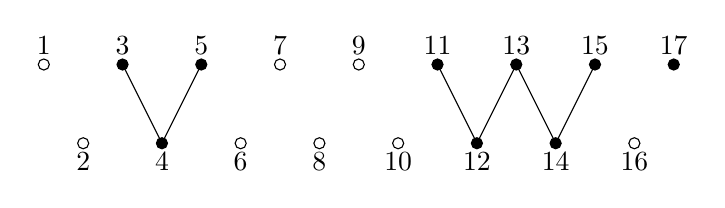
\begin{tikzpicture}
          \foreach \i in {3,5,11,13,15,17}{
            \draw[fill=black] (0.5*\i,1) circle (2pt);
            \node[above] at (0.5*\i,1) {\i};}
          \foreach \i in {1,7,9}{
            \draw[fill=white] (0.5*\i,1) circle (2pt);
            \node[above] at (0.5*\i,1) {\i};}
          \foreach \i in {4,12,14}{
            \draw[fill=black] (0.5*\i,0) circle (2pt);
            \draw (0.5*\i,0) -- (0.5*\i-0.5,1);
            \draw (0.5*\i,0) -- (0.5*\i+0.5,1);
            \node[below] at (0.5*\i,0) {\i};}
          \foreach \i in {2,6,8,10,16}{
            \draw[fill=white] (0.5*\i,0) circle (2pt);
            \node[below] at (0.5*\i,0) {\i};}
        \end{tikzpicture}
      \]
      The possible isomorphisms $\gamma$ with positive weight are given by
      \[
        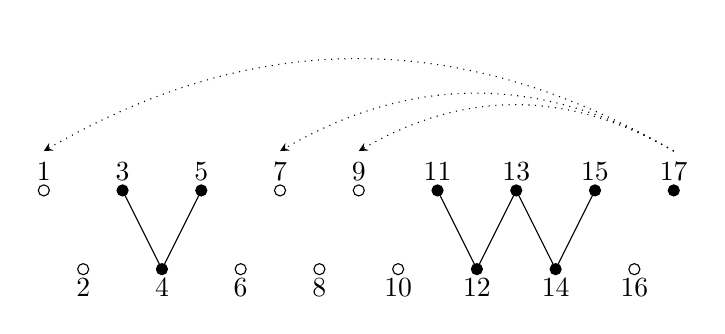
\begin{tikzpicture}
          \draw[dotted,-stealth] (8.5,1.5) to[out=150,in=30] (0.5,1.5);
          \draw[dotted,-stealth] (8.5,1.5) to[out=150,in=30] (3.5,1.5);
          \draw[dotted,-stealth] (8.5,1.5) to[out=150,in=30] (4.5,1.5);
          \foreach \i in {3,5,11,13,15,17}{
            \draw[fill=black] (0.5*\i,1) circle (2pt);
            \node[above] at (0.5*\i,1) {\i};}
          \foreach \i in {1,7,9}{
            \draw[fill=white] (0.5*\i,1) circle (2pt);
            \node[above] at (0.5*\i,1) {\i};}
          \foreach \i in {4,12,14}{
            \draw[fill=black] (0.5*\i,0) circle (2pt);
            \draw (0.5*\i,0) -- (0.5*\i-0.5,1);
            \draw (0.5*\i,0) -- (0.5*\i+0.5,1);
            \node[below] at (0.5*\i,0) {\i};}
          \foreach \i in {2,6,8,10,16}{
            \draw[fill=white] (0.5*\i,0) circle (2pt);
            \node[below] at (0.5*\i,0) {\i};}
        \end{tikzpicture}
      \]
      \[
        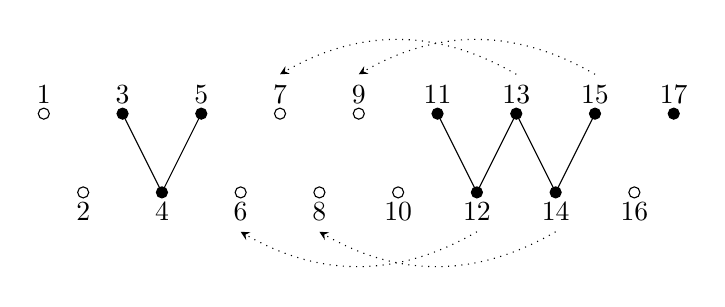
\begin{tikzpicture}
          \draw[dotted,-stealth] (6.5,1.5) to[out=150,in=30] (3.5,1.5);
          \draw[dotted,-stealth] (7.5,1.5) to[out=150,in=30] (4.5,1.5);
          \draw[dotted,-stealth] (6,-0.5) to[out=210,in=-30] (3,-0.5);
          \draw[dotted,-stealth] (7,-0.5) to[out=210,in=-30] (4,-0.5);
          \foreach \i in {3,5,11,13,15,17}{
            \draw[fill=black] (0.5*\i,1) circle (2pt);
            \node[above] at (0.5*\i,1) {\i};}
          \foreach \i in {1,7,9}{
            \draw[fill=white] (0.5*\i,1) circle (2pt);
            \node[above] at (0.5*\i,1) {\i};}
          \foreach \i in {4,12,14}{
            \draw[fill=black] (0.5*\i,0) circle (2pt);
            \draw (0.5*\i,0) -- (0.5*\i-0.5,1);
            \draw (0.5*\i,0) -- (0.5*\i+0.5,1);
            \node[below] at (0.5*\i,0) {\i};}
          \foreach \i in {2,6,8,10,16}{
            \draw[fill=white] (0.5*\i,0) circle (2pt);
            \node[below] at (0.5*\i,0) {\i};}
        \end{tikzpicture}
      \]
      \[
        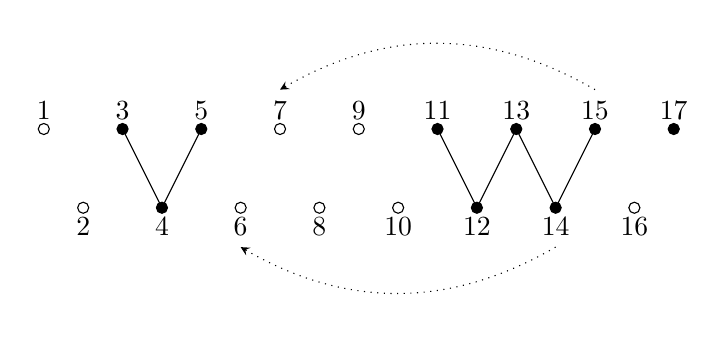
\begin{tikzpicture}
          \draw[dotted,-stealth] (7.5,1.5) to[out=150,in=30] (3.5,1.5);
          \draw[dotted,-stealth] (7,-0.5) to[out=210,in=-30] (3,-0.5);
          \foreach \i in {3,5,11,13,15,17}{
            \draw[fill=black] (0.5*\i,1) circle (2pt);
            \node[above] at (0.5*\i,1) {\i};}
          \foreach \i in {1,7,9}{
            \draw[fill=white] (0.5*\i,1) circle (2pt);
            \node[above] at (0.5*\i,1) {\i};}
          \foreach \i in {4,12,14}{
            \draw[fill=black] (0.5*\i,0) circle (2pt);
            \draw (0.5*\i,0) -- (0.5*\i-0.5,1);
            \draw (0.5*\i,0) -- (0.5*\i+0.5,1);
            \node[below] at (0.5*\i,0) {\i};}
          \foreach \i in {2,6,8,10,16}{
            \draw[fill=white] (0.5*\i,0) circle (2pt);
            \node[below] at (0.5*\i,0) {\i};}
        \end{tikzpicture}
      \]
      \[
        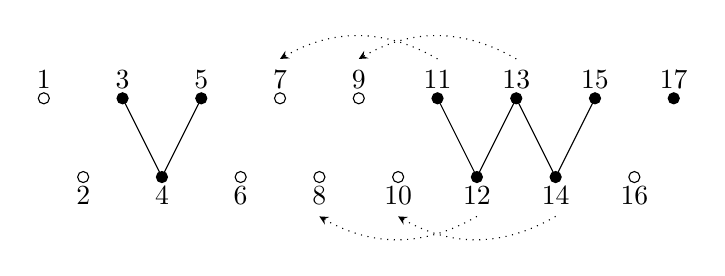
\begin{tikzpicture}
          \draw[dotted,-stealth] (5.5,1.5) to[out=150,in=30] (3.5,1.5);
          \draw[dotted,-stealth] (6.5,1.5) to[out=150,in=30] (4.5,1.5);
          \draw[dotted,-stealth] (6,-0.5) to[out=210,in=-30] (4,-0.5);
          \draw[dotted,-stealth] (7,-0.5) to[out=210,in=-30] (5,-0.5);
          \foreach \i in {3,5,11,13,15,17}{
            \draw[fill=black] (0.5*\i,1) circle (2pt);
            \node[above] at (0.5*\i,1) {\i};}
          \foreach \i in {1,7,9}{
            \draw[fill=white] (0.5*\i,1) circle (2pt);
            \node[above] at (0.5*\i,1) {\i};}
          \foreach \i in {4,12,14}{
            \draw[fill=black] (0.5*\i,0) circle (2pt);
            \draw (0.5*\i,0) -- (0.5*\i-0.5,1);
            \draw (0.5*\i,0) -- (0.5*\i+0.5,1);
            \node[below] at (0.5*\i,0) {\i};}
          \foreach \i in {2,6,8,10,16}{
            \draw[fill=white] (0.5*\i,0) circle (2pt);
            \node[below] at (0.5*\i,0) {\i};}
        \end{tikzpicture}
      \]
      \[
        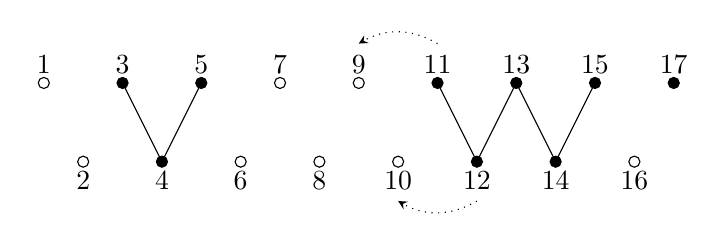
\begin{tikzpicture}
          \draw[dotted,-stealth] (5.5,1.5) to[out=150,in=30] (4.5,1.5);
          \draw[dotted,-stealth] (6,-0.5) to[out=210,in=-30] (5,-0.5);
          \foreach \i in {3,5,11,13,15,17}{
            \draw[fill=black] (0.5*\i,1) circle (2pt);
            \node[above] at (0.5*\i,1) {\i};}
          \foreach \i in {1,7,9}{
            \draw[fill=white] (0.5*\i,1) circle (2pt);
            \node[above] at (0.5*\i,1) {\i};}
          \foreach \i in {4,12,14}{
            \draw[fill=black] (0.5*\i,0) circle (2pt);
            \draw (0.5*\i,0) -- (0.5*\i-0.5,1);
            \draw (0.5*\i,0) -- (0.5*\i+0.5,1);
            \node[below] at (0.5*\i,0) {\i};}
          \foreach \i in {2,6,8,10,16}{
            \draw[fill=white] (0.5*\i,0) circle (2pt);
            \node[below] at (0.5*\i,0) {\i};}
        \end{tikzpicture}
      \]
      \[
        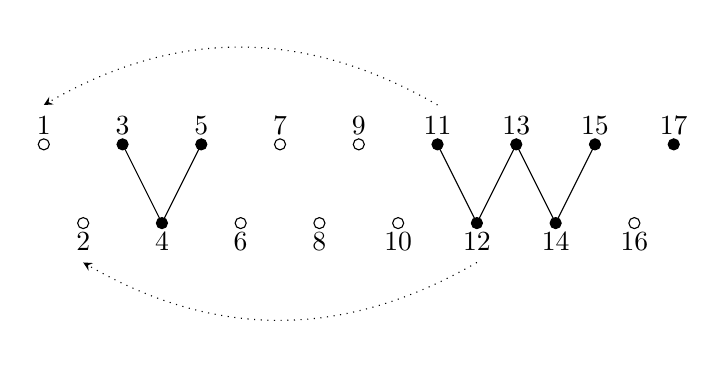
\begin{tikzpicture}
          \draw[dotted,-stealth] (5.5,1.5) to[out=150,in=30] (0.5,1.5);
          \draw[dotted,-stealth] (6,-0.5) to[out=210,in=-30] (1,-0.5);
          \foreach \i in {3,5,11,13,15,17}{
            \draw[fill=black] (0.5*\i,1) circle (2pt);
            \node[above] at (0.5*\i,1) {\i};}
          \foreach \i in {1,7,9}{
            \draw[fill=white] (0.5*\i,1) circle (2pt);
            \node[above] at (0.5*\i,1) {\i};}
          \foreach \i in {4,12,14}{
            \draw[fill=black] (0.5*\i,0) circle (2pt);
            \draw (0.5*\i,0) -- (0.5*\i-0.5,1);
            \draw (0.5*\i,0) -- (0.5*\i+0.5,1);
            \node[below] at (0.5*\i,0) {\i};}
          \foreach \i in {2,6,8,10,16}{
            \draw[fill=white] (0.5*\i,0) circle (2pt);
            \node[below] at (0.5*\i,0) {\i};}
        \end{tikzpicture}
      \]
      \[
        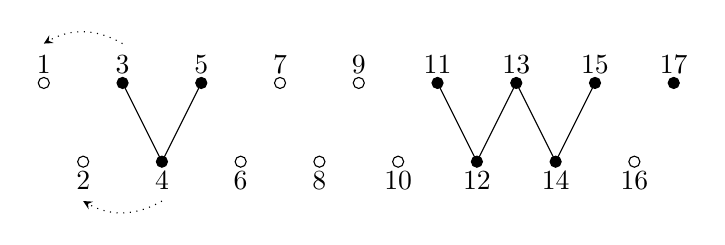
\begin{tikzpicture}
          \draw[dotted,-stealth] (1.5,1.5) to[out=150,in=30] (0.5,1.5);
          \draw[dotted,-stealth] (2,-0.5) to[out=210,in=-30] (1,-0.5);
          \foreach \i in {3,5,11,13,15,17}{
            \draw[fill=black] (0.5*\i,1) circle (2pt);
            \node[above] at (0.5*\i,1) {\i};}
          \foreach \i in {1,7,9}{
            \draw[fill=white] (0.5*\i,1) circle (2pt);
            \node[above] at (0.5*\i,1) {\i};}
          \foreach \i in {4,12,14}{
            \draw[fill=black] (0.5*\i,0) circle (2pt);
            \draw (0.5*\i,0) -- (0.5*\i-0.5,1);
            \draw (0.5*\i,0) -- (0.5*\i+0.5,1);
            \node[below] at (0.5*\i,0) {\i};}
          \foreach \i in {2,6,8,10,16}{
            \draw[fill=white] (0.5*\i,0) circle (2pt);
            \node[below] at (0.5*\i,0) {\i};}
        \end{tikzpicture}
      \]

    \end{example}

\section{Quiver Pl\"ucker Relations}
  Given a totally ordered set $K$, write $\epsilon(k,K)=\#\{k'\in K: k'\le k\}$.

  Consider the embedding $Gr_\bfe(P_m)\into Gr_{e_1}(\CC^m)\times Gr_{e_2}(\CC^{m-1})\into \PP^{{m \choose e_1} - 1}\times \PP^{{m-1 \choose e_2} - 1}$ which is the composition of the natural inclusion $Gr_\bfe(P_m)\into Gr_{e_1}(\CC^m)\times Gr_{e_2}(\CC^{m-1})$ with the Pl\"ucker embeddings of the ordinary Grassmannians according to the basis $\{v_{m,1},\cdots,v_{m,2m-1}\}$ of $P_m$.
  Then $Gr_\bfe(P_m)$ may be described explicitly in terms of the Pl\"ucker coordinates
  \[[\Delta_I:\Delta_J]_{I\subseteq_{e_1} \{2\ell-1\}, J\subseteq_{e_2} \{2\ell\}}.\]

  Indeed, since $Gr_\bfe(P_m)$ lies inside $Gr_{e_1}(\CC^m)\times Gr_{e_2}(\CC^{m-1})$, the ordinary Pl\"ucker relations must be satisfied:
  \[\sum_{i\in I'\setminus I} (-1)^{\epsilon(i,I)} \Delta_{I\cup\{i\}} \Delta_{I'\setminus\{i\}}=0
    \qquad
    \sum_{j\in J'\setminus J} (-1)^{\epsilon(j,J)} \Delta_{J\cup\{j\}} \Delta_{J'\setminus\{j\}}=0\]
  for each $I,I'\subseteq\{2\ell-1\}$ with cardinalities $e_1-1,e_1+1$ respectively and each $J,J'\subseteq\{2\ell\}$ with cardinalities $e_2-1,e_2+1$ respectively.
  In addition, the \emph{quiver Pl\"ucker relations} must be satisfied \cite{lorscheid-weist}:
  \begin{align}
    \label{eq:left Plucker} \sum_{j\in \{2\ell\}\setminus J} (-1)^{\epsilon(j-1,I)+\epsilon(j,J)} \Delta_{I\setminus\{j-1\}} \Delta_{J\cup\{j\}}=0,\\
    \label{eq:right Plucker} \sum_{j\in \{2\ell\}\setminus J} (-1)^{\epsilon(j+1,I)+\epsilon(j,J)} \Delta_{I\setminus\{j+1\}} \Delta_{J\cup\{j\}}=0,
  \end{align}
  for each $I\subseteq\{2\ell-1\}$ with cardinality $e_1+1$ and each $J\subseteq\{2\ell\}$ with cardinality $e_2-1$.
  In the equations above, we take $\Delta_I=0$ if $|I|=e_1+1$, i.e. when $j-1\notin I$ in \eqref{eq:left Plucker} or when $j+1\notin I$ in \eqref{eq:right Plucker}.
  \begin{remark}
    \label{rm:linear terms}
    Note that, upon restriction to an attractor cell $\AA_{S_1}^{S_2}$, each quiver Pl\"ucker relation has either zero, one, or two linear terms since the restriction imposes $\Delta_{S_1}=\Delta_{S_2}=1$.
    Thus necessary conditions for there to exist two linear terms in \eqref{eq:left Plucker} or \eqref{eq:right Plucker} are the containments $S_1\subseteq I$ and $J\subseteq S_2$.
    Moreover, this condition precludes the possibility that a constant appears in a restricted quiver Pl\"ucker relation since $I\setminus\{j\pm1\}\equiv S_1$ and $J\cup\{j\}\equiv S_2$ are incompatible with the successor-closed requirement for the subquiver $S_1\sqcup S_2$ to label a cell in $Gr_\bfe(P_m)$.
  \end{remark}

  \begin{lemma}
    The quiver Pl\"ucker relations \eqref{eq:left Plucker} and \eqref{eq:right Plucker} are invariant under the $\CC^*$-action on $Gr_\bfe(P_m)$
  \end{lemma}

  \subsection{Torus action on $\CC[Gr_\bfe(P_m)]$}
  The action of $\CC^*$ on $Gr_\bfe(P_m)$ induces an action on the quiver Pl\"ucker coordinates $\Delta_I$, $\Delta_J$ for $I\subseteq_{e_1} \{2k-1\}$ and $J\subseteq_{e_2} \{2k\}$.


  \subsection{Restriction to Cells}

  \begin{lemma}
    Let $S_1\sqcup S_2$ be a successor-closed subset of the support quiver of $\tilde P_m$ with $|S_i|=e_i$.
    Given $I \subseteq_{e_1} \{2\ell-1\}$ (resp. $J \subseteq_{e_2} \{2\ell\}$), we have $\Delta_I\equiv 0$ (resp. $\Delta_J\equiv 0$) when restricted to the attractor cell $\AA_{S_1}^{S_2}$ if there exists $t\in I\setminus S_1$ such that $\#\{s\in S_1:s\notin I, s>t\} < \#\{s\in I:s\notin S_1, s \ge t\}$ (and similarly for $J$).
  \end{lemma}
  \begin{proof}
    This matches the same condition for vanishing of Pl\"ucker coordinates in ordinary Schubert cells.
  \end{proof}
  \begin{corollary}
    Let $S_1\sqcup S_2$ be a successor-closed subset of the support quiver of $\tilde P_m$ with $|S_i|=e_i$.
    Given $I \subseteq_{e_1} \{2\ell-1\}$ with $S_1<I$ (resp. $J \subseteq_{e_2} \{2\ell\}$ with $S_2<J$), in reverse lexicographic ordering, we have $\Delta_I \equiv 0$ (resp. $\Delta_J\equiv 0$) when restricted to the attractor cell $\AA_{S_1}^{S_2}$.
  \end{corollary}

  The following describes those quiver Pl\"ucker relations with two linear terms over $\AA_{S_1}^{S_2}$.
  \begin{lemma}
    Let $S_1\sqcup S_2$ be a successor-closed subset of the support quiver of $\tilde P_m$ with associated fixed point $E$ and $\bar{S}_1\sqcup\bar{S}_2$ the predecessor-closed subset associated with $P_m/E$.
    The subsets $I\subseteq\{2\ell-1\}$ with cardinality $e_1+1$ and $J\subseteq\{2\ell\}$ with cardinality $e_2-1$ for which the quiver Pl\"ucker relation \eqref{eq:left Plucker} (resp. \eqref{eq:right Plucker}) has two linear terms are precisely those of the form
    \[I=S_1\cup\{\sigma_\ell(s-1)\} \qquad \text{and} \qquad J=S_2\setminus\{s\}\]
    (resp. $I=S_1\cup\{\sigma_\ell(s+1)\}$ and $J=S_2\setminus\{s\}$), where $s\in S_2$ and $\sigma_\ell(t)=t-\ell$ for $\ell\ge1$ with $\sigma_\ell(s)\in\bar{S}_2$ and $\sigma_\ell(s-1)\in\bar{S}_1$ (resp. $\sigma_\ell(s+1)\in\bar{S}_1$).
    In this case, quiver Pl\"ucker relation \eqref{eq:left Plucker} (resp. \eqref{eq:right Plucker}) contains the two linear terms $\Delta_{I\setminus\{s-1\}\cup\{\sigma_\ell(s-1)\}}$ (resp. $\Delta_{I\setminus\{s+1\}\cup\{\sigma_\ell(s+1)\}}$) and $\Delta_{J\setminus\{s\}\cup\{\sigma_\ell(s)\}}$.
  \end{lemma}
  \begin{proof}
    Observe first that indeed the quiver Pl\"ucker relations given above have two linear terms since $s\pm1\in S_1$ for $s\in S_2$ while the conditions on the shift $\ell$ imply $\sigma_\ell(s\pm1)\notin S_1$ and $\sigma_\ell(s)\notin S_2$ with $\Delta_{S_1\setminus\{s\pm1\}\cup\{\sigma_\ell(s\pm1)\}}$ and $\Delta_{S_2\setminus\{s\}\cup\{\sigma_\ell(s)\}}$ not identically zero on $\AA_{S_1}^{S_2}$.

    Now consider subsets $I$ and $J$ with $S_1\subseteq I$ and $J\subseteq S_2$ for which a quiver Pl\"ucker relation \eqref{eq:left Plucker} or \eqref{eq:right Plucker} has two linear terms.
    Set $\varepsilon=-1$ if this relation comes from \eqref{eq:left Plucker} and set $\varepsilon=+1$ if this relation comes from \eqref{eq:right Plucker}.
    Let $t+\varepsilon$ denote the unique element in $I\setminus S_1$ and let $s$ denote the unique element in $S_2\setminus J$.
    By assumption, the term $\Delta_{I\setminus\{t+\varepsilon\}} \Delta_{J\cup\{t\}}$ must be linear and so the minor $\Delta_{J\cup\{t\}}$ cannot be identically zero nor identically one on $\AA_{S_1}^{S_2}$ following Remark~\ref{rm:linear terms}.
    This forces $t<s$ and $t\in\bar{S_2}$.
    Similar consideration with the term $\Delta_{I\setminus\{s+\varepsilon\}} \Delta_{J\cup\{s\}}$ show that $s+\varepsilon\in\bar{S}_1$.
    Thus we may set $\ell=s-t$ and construct the sets $I$ and $J$ as above.
  \end{proof}

  The next two results describe those quiver Pl\"ucker relations with only one linear term over $\AA_{S_1}^{S_2}$.
  \begin{lemma}
    Upon restriction to $\AA_{S_1}^{S_2}$, a minor $\Delta_I$ (resp. $\Delta_J$) is the sole linear term in a quiver Pl\"ucker relation if it is not identically zero on $\AA_{S_1}^{S_2}$ and differs from $S_1$ (resp. $S_2$) in at least two places.
  \end{lemma}

  \begin{lemma}
    Let $S_1\sqcup S_2$ be a successor-closed subset of the support quiver of $\tilde P_m$ with $|S_i|=e_i$.
    Given $I \subseteq_{e_1} \{2\ell-1\}$ (resp. $J \subseteq_{e_2} \{2\ell\}$) with $|I\setminus S_1|\ge2$ and $\Delta_I\not\equiv 0$ on $\AA_{S_1}^{S_2}$ (resp. $|J\setminus S_2|\ge 2$ and $\Delta_J\not\equiv 0$ on $\AA_{S_1}^{S_2}$), there exists a standard Pl\"ucker relation in which $\Delta_I$ (resp. $\Delta_J$) is the sole linear term.
    Moreover, in any such Pl\"ucker relation every other Pl\"ucker coordinate $\Delta_{I'}$ (resp. $\Delta_{J'}$) appearing in the relation satisfies $I<I'$ (resp. $J<J'$) in the reverse lexicographic ordering.
  \end{lemma}
  \begin{lemma}
    \mbox{}
    \begin{enumerate}
      \item For every lift of an arrow of $Q$ to $S_1\sqcup S_2$ and to $\bar{S}_1\sqcup \bar{S}_2$, there exists a unique minimal expansion to a pair consisting of a connected predecessor-closed subquiver $\Gamma_E$ of $S_1\sqcup S_2$ and a connected successor-closed subquiver $\Gamma_{P_m/E}$ of $\bar{S}_1\sqcup \bar{S}_2$ each containing the respective lifted arrow with a corresponding (partial) isomorphism $\gamma:\Gamma_E\to\Gamma_{P_m/E}$.
      \item If the expansions $\Gamma_E$ and $\Gamma_{P_m/E}$ are not isomorphic quivers, then the following hold:
        \begin{enumerate}
          \item $1=\gamma(s+1)$ for some $s+1\in S_1$;
          \item $\gamma$ is surjective;
          \item the minor $\Delta_{S_1\setminus\{s+1\}\cup\{1\}}$ appears as the sole linear term in a quiver Pl\"ucker relation, where $s+1$ is the vertex of $\Gamma_E$ identified with vertex $1$ of $\Gamma_{P_m/E}$ under the bijection of vertices coming from the expansion procedure;
          \item none of the minors associated to $\gamma$ are necessary to parametrize the cell $\AA_{S_1}^{S_2}$.
        \end{enumerate}
    \end{enumerate}
  \end{lemma}
  \begin{proof}
    Take $I=S_1\cup\{1\}$ and $J=S_2\setminus\{s\}$ in the quiver Pl\"ucker relation \eqref{eq:right Plucker}.
  \end{proof}

  \begin{lemma}
    Let $S_1\sqcup S_2$ be a successor-closed subset of the support quiver of $\tilde P_m$ with associated $\CC^*$-fixed point $E\in Gr_\bfe(P_m)$.
    Given any isomorphism $\gamma:\Gamma_E\to\Gamma_{P_m/E}$ as in Section~\ref{sec:tangent parametrization}, say with
    \[\Gamma_E=\{v_{m,t},v_{m,t+1},\ldots,v_{m,t+\ell}\}\qquad\text{and}\qquad\Gamma_{P_m/E}=\{v_{m,t'},v_{m,t'+1},\ldots,v_{m,t'+\ell}\}\]
    such that $t'<t$ and $\ell>0$, the following hold:
    \begin{enumerate}
      \item there exists a quiver Pl\"ucker relation which, upon restriction to $\AA_{S_1}^{S_2}$, takes the form
        \[\Delta_{S_1\setminus\{s-1\}\cup\{\gamma(s-1)\}}-\varepsilon_\gamma(s)\Delta_{S_2\setminus\{s\}\cup\{\gamma(s)\}}=homogeneous~quadratic\]
        whenever $s$ is even with $t<s\le t+\ell$;
      \item there exists a quiver Pl\"ucker relation which, upon restriction to $\AA_{S_1}^{S_2}$, takes the form
        \[\Delta_{S_1\setminus\{s+1\}\cup\{\gamma(s+1)\}}-\varepsilon'_\gamma(s)\Delta_{S_2\setminus\{s\}\cup\{\gamma(s)\}}=homogeneous~quadratic\]
        whenever $s$ is even with $t\le s<t+\ell$.
    \end{enumerate}
  \end{lemma}
  \begin{proof}
    Observe that $\Delta_{S_1}=\Delta_{S_2}=1$ on $\AA_{S_1}^{S_2}$.
    Take $I=S_1\cup\{\gamma(s-1)\}$ and $J=S_2\setminus\{s\}$ in equation \eqref{eq:left Plucker} for $s$ even with $t<s\le t+\ell$ to get part (1).
    Take $I=S_1\cup\{\gamma(s+1)\}$ and $J=S_2\setminus\{s\}$ in equation \eqref{eq:right Plucker} for $s$ even with $t\le s<t+\ell$ to get part (2).
  \end{proof}

  \begin{lemma}
    Let $S_1\sqcup S_2$ be a successor-closed subset of the support quiver of $\tilde P_m$ with associated fixed point $E$.
    There exists $I\subseteq\{2\ell-1\}$ with cardinality $e_1+1$ and each $J\subseteq\{2\ell\}$ with cardinality $e_2-1$ such that $S_1\subseteq I$ and $J\subseteq S_2$ if and only if
  \end{lemma}

  \begin{theorem}
    Let $S_1\sqcup S_2$ be a successor-closed subset of the support quiver of $\tilde P_m$ with $|S_i|=e_i$.
    Then the attractor cell $\AA_{S_1}^{S_2}$ is parametrized as an affine space by the Pl\"ucker coordinates
    \begin{itemize}
      \item $\Delta_J$ for $J=S_2\setminus\{s\}\cup\{t\}$ with $s\in S_2$, $t\in\bar{S}_2$, and $t<s$;
      \item $\Delta_I$ for $I=???$
    \end{itemize}
  \end{theorem}
  \begin{proof}
    By construction, upon restriction to $\AA_{S_1}^{S_2}$ we have $\Delta_{S_1}\equiv 1$, $\Delta_{S_2}\equiv 1$.
    Also,
    \[\Delta_I\equiv 0 \qquad \Delta_J\equiv 0\]
    if there exists $i\in I\setminus S_1$ such that $\#\{j\in S_1:j\notin I, j>i\} < \#\{j\in I:j\notin S_1,j>i\}$ and similarly for $J$.
  \end{proof}

\section{Cell Closure Properties}

  \begin{itemize}
    \item Suppose $U\in\AA_{S_1}^{S_2}$ and $V\in\overline{\AA}_{S_1}^{S_2}\setminus\AA_{S_1}^{S_2}$.
      What can be said about $\Hom(U,V)$ and $\Hom(V,U)$?
  \end{itemize}

  Let $\bfe\in\ZZ^2$.
  Write $\cC_\bfe$ for the set of all compatible pairs $(S_1,S_2)$ with $S_1 \subseteq_{e_1} \{2k\}$ and $S_2 \subseteq_{e_2} \{2k+1\}$.
  We consider the lexicographic ordering $\prec$ on $\cC_\bfe$, i.e. $(S'_1,S'_2) \prec (S_1,S_2)$ if $S'_1 < S_1$ or $S'_1 = S_1$ and $S'_2 < S_2$, where $<$ denotes the standard lexicographic ordering on subsets.
  \begin{theorem}
    For any $(S_1,S_2)\in\cC_\bfe$, the set $\bigsqcup\limits_{(S'_1,S'_2)\preceq (S_1,S_2)} A_{S'_1}^{S'_2}$ is closed in $Gr_\bfe(P_n)$.
  \end{theorem}
  \begin{proof}
    We show by induction along the ordering $\prec$ on $\cC_\bfe$ that
    \[\overline{\AA}_{S_1}^{S_2}\subset\bigsqcup\limits_{(S'_1,S'_2)\preceq (S_1,S_2)} A_{S'_1}^{S'_2}.\]
    Since $\AA_{1,\ldots,2e_1-1}^{2,\ldots,2e_2}$ is just a point and is initial in $\cC_\bfe$, there is nothing to show.

    For any other $(S_1,S_2) \in \cC_\bfe$, we clearly have $\AA_{S_1}^{S_2} \subset \overline{\AA}_{S_1}^{S_2}$, so we consider $(S'_1,S'_2)\prec (S_1,S_2)$.
    If $S'_1=S_1$, then $\AA_{S'_1}^{S'_2} \subset \overline{\AA}_{S_1}^{S_2}$ along the same degeneration giving $\AA_{S'_2}$ on the boundary of $\AA_{S_2}$ inside $Gr_{e_2}(\CC^n)$.
    Similarly, when $S'_2=S_2$, the intersection of $\overline{\AA}_{S_1}^{S_2}$ with $\AA_{S'_1}^{S'_2}$ occurs along the degeneration giving $\AA_{S'_1}$ on the boundary of $\AA_{S_1}$ inside $Gr_{e_1}(\CC^{n+1})$, but imposes relations on the image of its projection into $\AA_{S_2}$ inside $Gr_{e_2}(\CC^n)$.

    Now suppose $(S'_1,S'_2) \prec (S_1,S_2)$ with $S'_1 < S_1$ and $S'_2 < S_2$.
    \sayDR{Completing this proof requires some combinatorics that I haven't worked out yet.}
  \end{proof}

  \begin{example}
    The quiver Grassmannian $Gr_{(4,2)}(P_5)$ is defined as a subscheme of $Gr_4(\CC^5)\times Gr_2(\CC^4)$ via the quiver Pl\"ucker relations in the standard Pl\"ucker coordinates:
    \begin{align*}
      0 &= \Delta_{3,5,7,9} \Delta_{2,8} - \Delta_{1,5,7,9}\Delta_{4,8} + \Delta_{1,3,7,9}\Delta_{6,8}\\
      0 &= \Delta_{1,5,7,9}\Delta_{2,8} - \Delta_{1,3,7,9}\Delta_{4,8} + \Delta_{1,3,5,9}\Delta_{6,8}\\
      0 &= \Delta_{3,5,7,9} \Delta_{2,6} - \Delta_{1,5,7,9}\Delta_{4,6} + \Delta_{1,3,5,9}\Delta_{6,8}\\
      0 &= \Delta_{1,5,7,9}\Delta_{2,6} - \Delta_{1,3,7,9}\Delta_{4,6} + \Delta_{1,3,5,7}\Delta_{6,8}\\
      0 &= \Delta_{3,5,7,9} \Delta_{2,4} - \Delta_{1,3,7,9}\Delta_{4,6} + \Delta_{1,3,5,9}\Delta_{4,8}\\
      0 &= \Delta_{1,5,7,9}\Delta_{2,4} - \Delta_{1,3,5,9}\Delta_{4,6} + \Delta_{1,3,5,7}\Delta_{4,8}\\
      0 &= \Delta_{1,5,7,9}\Delta_{2,4} - \Delta_{1,3,7,9}\Delta_{2,6} + \Delta_{1,3,5,9}\Delta_{2,8}\\
      0 &= \Delta_{1,3,7,9}\Delta_{2,4} - \Delta_{1,3,5,9}\Delta_{2,6} + \Delta_{1,3,5,7}\Delta_{2,8}
    \end{align*}
    Observe that this collection of relations is invariant under the action of the longest element in the symmetric group $\Sigma_9$.
    Together with the standard Pl\"ucker relation on $Gr_2(\CC^4)$:
    \begin{equation*}
      0 = \Delta_{4,6}\Delta_{2,8} - \Delta_{4,8}\Delta_{2,6} + \Delta_{6,8}\Delta_{2,4},
    \end{equation*}
    we obtain all of the relations for the quiver Grassmannian $Gr_{(4,2)}(P_5)$ in the Pl\"ucker embedding.

    Using these, we compute the closures of the affine cells $\AA_{S_1}^{S_2}$ in order of increasing dimension.
    \begin{itemize}
      \item $S_1=\{1,3,5,7\}$, $S_2=\{2,4\}$: The cell $\AA_{1,3,5,7}^{2,4}$ is just a point where all relations vanish.

      \item $S_1=\{1,3,5,7\}$, $S_2=\{2,6\}$: The cell $\AA_{1,3,5,7}^{2,6} \cong \AA^1$ has coordinate $\Delta_{2,4}$ and where all relations vanish.
        The closure contains:
        \begin{itemize}
          \item the cell $\AA_{1,3,5,7}^{2,4}$ in the limit $|\Delta_{2,4}|\to\infty$;
        \end{itemize}
        and identifies with $\PP^1$ via the projection to $Gr_2(\CC^4)$.

      \item $S_1=\{1,3,5,7\}$, $S_2=\{4,6\}$: The cell $\AA_{1,3,5,7}^{4,6} \cong \AA^2$ is an affine plane with Pl\"ucker coordinates $\Delta_{2,4},\Delta_{2,6}$ and where all relations vanish.
        The closure contains:
        \begin{itemize}
          \item the cell $\AA_{1,3,5,7}^{2,6}$ in the limit $|\Delta_{2,6}|\to\infty$ with $\Delta_{2,4}/\Delta_{2,6}$ as coordinate;
          \item the cell $\AA_{1,3,5,7}^{2,4}$ in the limit $|\Delta_{2,4}/\Delta_{2,6}|\to\infty$;
        \end{itemize}
        and identifies with $\PP^2$ via the projection to $Gr_2(\CC^4)$.

      \item $S_1=\{1,3,5,9\}$, $S_2=\{2,4\}$: The cell $\AA_{1,3,5,9}^{2,4} \cong \AA^1$ is an affine line with Pl\"ucker coordinate $\Delta_{1,3,5,7}$ and where all relations vanish.
        The closure contains:
        \begin{itemize}
          \item the cell $\AA_{1,3,5,7}^{2,4}$ in the limit $|\Delta_{1,3,5,7}|\to\infty$
        \end{itemize}
        and identifies with $\PP^1$ via the projection to $Gr_4(\CC^5)$.

      \item $S_1=\{1,3,7,9\}$, $S_2=\{2,8\}$: The cell $\AA_{1,3,7,9}^{2,8} \cong \AA^2$ is an affine plane with Pl\"ucker coordinates $\Delta_{1,3,5,7}$, $\Delta_{1,3,5,9}$, $\Delta_{2,4}$, $\Delta_{2,6}$ satisfying the relations:
        \begin{align*}
           0 &=  - \Delta_{2,6} + \Delta_{1,3,5,9}\\
           0 &= \Delta_{2,4} - \Delta_{1,3,5,9}\Delta_{2,6} + \Delta_{1,3,5,7}
        \end{align*}
        The closure contains:
        \begin{itemize}
          \item the cell $\AA_{1,3,5,7}^{2,6}$ in the limit $|\Delta_{2,6}|\to\infty$ with $\Delta_{2,4}/\Delta_{2,6}$ as coordinate (note that $|\Delta_{1,3,5,7}/\Delta_{1,3,5,9}|\to\infty$ in the limit);
          \item the cell $\AA_{1,3,5,9}^{2,4}$
          \item the cell $\AA_{1,3,5,7}^{2,4}$
        \end{itemize}
        the union of which identifies with the blow-up of $\overline{\AA}_{1,3,5,7}^{2,6}$ at the point $\AA_{1,3,5,7}^{2,4}$ with special fiber $\overline{\AA}_{1,3,5,9}^{2,4}$.
        After projecting the closure to $Gr_4(\CC^5)$, we obtain the copy of $\PP^2$ given by $\overline{\AA}_{2,8}$.
        However, the fiber over the point $\AA_{2,4}$ is given by $\overline{\AA}_{1,3,5,9}^{2,4}$.
        In this way, $\overline{\AA}_{1,3,7,9}^{2,8}$ is obtained by gluing $\AA_{1,3,7,9}^{2,8}$ onto the blow-up of $\overline{\AA}_{1,3,5,7}^{2,6}$ at the point $\AA_{1,3,5,7}^{2,4}$.

      \item $S_1=\{3,5,7,9\}$, $S_2=\{4,6\}$: The cell $\AA_{3,5,7,9}^{4,6} \cong \AA^2$ is two-dimensional with Pl\"ucker coordinates $\Delta_{1,3,5,7}$, $\Delta_{1,3,5,9}$, $\Delta_{1,3,7,9}$, $\Delta_{1,5,7,9}$, $\Delta_{2,4}$, $\Delta_{2,6}$ satisfying the relations:
        \begin{align*}
          0 &= \Delta_{2,6} - \Delta_{1,5,7,9}\\
          0 &= \Delta_{1,5,7,9}\Delta_{2,6} - \Delta_{1,3,7,9}\\
          0 &= \Delta_{2,4} - \Delta_{1,3,7,9}\\
          0 &= \Delta_{1,5,7,9}\Delta_{2,4} - \Delta_{1,3,5,9}\\
          0 &= \Delta_{1,5,7,9}\Delta_{2,4} - \Delta_{1,3,7,9}\Delta_{2,6}\\
          0 &= \Delta_{1,3,7,9}\Delta_{2,4} - \Delta_{1,3,5,9}\Delta_{2,6}
        \end{align*}
        The closure contains:
        \begin{itemize}
          \item the curve $\langle \Delta_{2,4}=\Delta_{2,6}^2 \rangle \subset \AA_{1,3,5,7}^{4,6}$ in the limit $|\Delta_{1,3,5,7}|\to\infty$
          \item the cell $\AA_{1,3,5,9}^{2,4}$ in the limit $|\Delta_{2,6}|\to\infty$ with $\frac{\Delta_{1,3,5,7}}{\Delta_{1,3,5,9}}$ as coordinate
          \item the cell $\AA_{1,3,5,7}^{2,4}$ in the limit $|\frac{\Delta_{1,3,5,7}}{\Delta_{1,3,5,9}}|\to\infty$ since $|\Delta_{2,6}^3|\equiv|\Delta_{1,3,5,9}|\to\infty$ implies $|\Delta_{2,4}/\Delta_{2,6}|\to\infty$
        \end{itemize}

      \item $S_1=\{1,5,7,9\}$, $S_2=\{6,8\}$: The cell $\AA_{1,5,7,9}^{6,8} \cong \AA^3$ is three-dimensional with Pl\"ucker coordinates $\Delta_{1,3,5,7}$, $\Delta_{1,3,5,9}$, $\Delta_{1,3,7,9}$, $\Delta_{2,4}$, $\Delta_{2,6}$, $\Delta_{2,8}$, $\Delta_{4,6}$, $\Delta_{4,8}$ satisfying the relations:
      \begin{align*}
        0 &= -\Delta_{4,8} + \Delta_{1,3,7,9}\\
        0 &= \Delta_{2,8} - \Delta_{1,3,7,9}\Delta_{4,8} + \Delta_{1,3,5,9}\\
        0 &= -\Delta_{4,6} + \Delta_{1,3,5,9}\\
        0 &= \Delta_{2,6} - \Delta_{1,3,7,9}\Delta_{4,6} + \Delta_{1,3,5,7}\\
        0 &= - \Delta_{1,3,7,9}\Delta_{4,6} + \Delta_{1,3,5,9}\Delta_{4,8}\\
        0 &= \Delta_{2,4} - \Delta_{1,3,5,9}\Delta_{4,6} + \Delta_{1,3,5,7}\Delta_{4,8}\\
        0 &= \Delta_{2,4} - \Delta_{1,3,7,9}\Delta_{2,6} + \Delta_{1,3,5,9}\Delta_{2,8}\\
        0 &= \Delta_{1,3,7,9}\Delta_{2,4} - \Delta_{1,3,5,9}\Delta_{2,6} + \Delta_{1,3,5,7}\Delta_{2,8}
      \end{align*}

      \item $S_1=\{3,5,7,9\}$, $S_2=\{4,8\}$: The cell $\AA_{3,5,7,9}^{4,8} \cong \AA^3$ is three-dimensional with Pl\"ucker coordinates $\Delta_{1,3,5,7}$, $\Delta_{1,3,5,9}$, $\Delta_{1,3,7,9}$, $\Delta_{1,5,7,9}$, $\Delta_{2,4}$, $\Delta_{2,6}$, $\Delta_{2,8}$, $\Delta_{4,6}$ satisfying the relations:
      \begin{align*}
        0 &= \Delta_{2,8} - \Delta_{1,5,7,9} + \Delta_{1,3,7,9}\Delta_{6,8}\\
        0 &= \Delta_{1,5,7,9}\Delta_{2,8} - \Delta_{1,3,7,9} + \Delta_{1,3,5,9}\Delta_{6,8}\\
        0 &= \Delta_{2,6} - \Delta_{1,5,7,9}\Delta_{4,6} + \Delta_{1,3,5,9}\Delta_{6,8}\\
        0 &= \Delta_{1,5,7,9}\Delta_{2,6} - \Delta_{1,3,7,9}\Delta_{4,6} + \Delta_{1,3,5,7}\Delta_{6,8}\\
        0 &= \Delta_{2,4} - \Delta_{1,3,7,9}\Delta_{4,6} + \Delta_{1,3,5,9}\\
        0 &= \Delta_{1,5,7,9}\Delta_{2,4} - \Delta_{1,3,5,9}\Delta_{4,6} + \Delta_{1,3,5,7}\\
        0 &= \Delta_{1,5,7,9}\Delta_{2,4} - \Delta_{1,3,7,9}\Delta_{2,6} + \Delta_{1,3,5,9}\Delta_{2,8}\\
        0 &= \Delta_{1,3,7,9}\Delta_{2,4} - \Delta_{1,3,5,9}\Delta_{2,6} + \Delta_{1,3,5,7}\Delta_{2,8}
      \end{align*}

      \item $S_1=\{3,5,7,9\}$, $S_2=\{6,8\}$: The cell $\AA_{3,5,7,9}^{6,8} \cong \AA^4$ is four-dimensional with Pl\"ucker coordinates $\Delta_{1,3,5,7}$, $\Delta_{1,3,5,9}$, $\Delta_{1,3,7,9}$, $\Delta_{1,5,7,9}$, $\Delta_{2,4}$, $\Delta_{2,6}$, $\Delta_{2,8}$, $\Delta_{4,6}$, $\Delta_{4,8}$ satisfying the relations:
      \begin{align*}
        0 &= \Delta_{2,8} - \Delta_{1,5,7,9}\Delta_{4,8} + \Delta_{1,3,7,9}\\
        0 &= \Delta_{1,5,7,9}\Delta_{2,8} - \Delta_{1,3,7,9}\Delta_{4,8} + \Delta_{1,3,5,9}\\
        0 &= \Delta_{2,6} - \Delta_{1,5,7,9}\Delta_{4,6} + \Delta_{1,3,5,9}\\
        0 &= \Delta_{1,5,7,9}\Delta_{2,6} - \Delta_{1,3,7,9}\Delta_{4,6} + \Delta_{1,3,5,7}\\
        0 &= \Delta_{2,4} - \Delta_{1,3,7,9}\Delta_{4,6} + \Delta_{1,3,5,9}\Delta_{4,8}\\
        0 &= \Delta_{1,5,7,9}\Delta_{2,4} - \Delta_{1,3,5,9}\Delta_{4,6} + \Delta_{1,3,5,7}\Delta_{4,8}\\
        0 &= \Delta_{1,5,7,9}\Delta_{2,4} - \Delta_{1,3,7,9}\Delta_{2,6} + \Delta_{1,3,5,9}\Delta_{2,8}\\
        0 &= \Delta_{1,3,7,9}\Delta_{2,4} - \Delta_{1,3,5,9}\Delta_{2,6} + \Delta_{1,3,5,7}\Delta_{2,8}
      \end{align*}
    \end{itemize}
  \end{example}

% \section{Approach 2: Caldero-Chapoton Fibrations}
% Given a short exact sequence
% \[\begin{tikzcd}
%   0 \arrow{r} & M \arrow["\iota"]{r} & B \arrow["\pi"]{r} & N \arrow{r} & 0
% \end{tikzcd}\]
% of representations, we get an induced map of quiver Grassmannians
% \begin{align*}
%   \Psi:Gr_\bfe(B) &\to \bigsqcup_{\bff+\bfg=\bfe} Gr_\bff(M)\times Gr_\bfg(N) \\
%   E &\mapsto \big(E\cap\iota(M),\pi(E)=(E+\iota(M))/\iota(M)\big)
% \end{align*}
% A result of Caldero and Chapoton shows that the fiber over a point $(F,G)$ in the image of $\Psi$ is isomorphic to the affine space $\Hom_Q(G,M/F)$.

% The difficulty of using these maps to inductively establish cell decompositions of quiver Grassmannians is in understanding the how these fiber dimensions vary over the image of $\Psi$.
% In our situation, these can be controlled for special short exact sequences:
% \[\begin{tikzcd}
%     0 \arrow{r} & P_m^{\alpha} \arrow["\alpha"]{r} & P_{m+1} \arrow{r} & D_\beta \arrow{r} & 0
% \end{tikzcd}\]
% for $m$ odd, where the dimension vector of $D_\beta$ is $(1,1)$ with $\alpha$ acting as zero and $\beta$ acting as the identity map, and
% \[\begin{tikzcd}
%     0 \arrow{r} & P_m^{\beta} \arrow["\beta"]{r} & P_{m+1} \arrow{r} & D_\beta \arrow{r} & 0
% \end{tikzcd}\]
% for $m$ even.
% \begin{lemma}
%   For any proper subrepresentation $G\subsetneq D_\beta$ and any subrepresentation $F\subseteq P_m$, the fiber $\Psi^{-1}(F,G)$ is non-empty
% \end{lemma}

\section{Future Directions}
  \begin{itemize}
    \item Find the classes of cells in cohomology with basis given by opposite cells (from the inverted torus action).
    \item Find the intersections of opposite cells.
    \item Study the cohomology classes of their closures.
  \end{itemize}

\begin{thebibliography}{10}

\bibitem{ass}
  I.~Assem, D.~Simson, A.~Skowronski: Elements of the Representation Theory of Associative Algebras. Cambridge University Press, Cambridge 2007.

\bibitem{ars}
  M.~Auslander, I.~Reiten, S.~O.~Smalo: Representation theory of Artin algebras {\bf 36}. Cambridge University Press, Cambridge 1997.

\bibitem{bb}
  A.~Bia\l{}ynicki-Birula: Some theorems on actions of algebraic groups. Annals of Mathematics \textbf{98}, 480-497 (1973).

\bibitem{bgp}
  I.~N.~Bernstein, I.~M.~Gelfand, V.~A.~Ponomarev: Coxeter functors, and Gabriel's theorem. Russian Mathematical Surveys \textbf{28}(2), 17-32 (1973).

\bibitem{brenner-butler}
  S.~Brenner, M.~C.~R.~Butler: The equivalence of certain functors occurring in the representation theory of artin algebras and species. Journal of the London Mathematical Society \textbf{2}(1), 183-187 (1976).

\bibitem{cc}
  P.~Caldero, F.~Chapoton: Cluster algebras as {H}all algebras of quiver representations. Commentarii Mathematici Helvetici \textbf{81}(3), 595-616 (2006).

\bibitem{ck}
  P.~Caldero, B.~Keller: From triangulated categories to cluster algebras II.  Annales Scientifique de l'Ecole Normale Superi\'{e}ure (4) \textbf{39} (6), 983-1009 (2006).

\bibitem{cr}
  P.~Caldero, M.~Reineke: On the quiver Grassmannian in the acyclic case. Journal of Pure and Applied Algebra \textbf{212}(11), 2369-2380 (2008).

\bibitem{ca}	J.B.~Carrell: Torus actions and cohomology. Algebraic quotients. Torus actions and cohomology. The adjoint representation and the adjoint action, 83-158. Encyclopaedia Mathematical Science \textbf{131}, Invariant Theory and Algebraic Transformation Groups, Springer, Berlin, 2002.

\bibitem{cerulli irelli-esposito}
  G.~Cerulli Irelli, F.~Esposito: Geometry of quiver Grassmannians of Kronecker type and applications to cluster algebras. Algebra \&  Number Theory \textbf{5}(6), 777-801 (2011).

\bibitem{cefr}
  G.~Cerulli Irelli, F.~Esposito, H.~Franzen, M.~Reineke: Topology of Quiver Grassmannians. Preprint 2018.

\bibitem{gab}
  P.~Gabriel: The universal cover of a finite-dimensional algebra. Representations of algebras. Lecture Notes in Mathematics {\bf 903}, 68-105 (1981).

\bibitem{llz}
  K.~Lee, L.~Li, A.~Zelevinsky: Greedy elements in rank 2 cluster algebras. Selecta Mathematica \textbf{20}(1), 57-82 (2014).

\bibitem{lorscheid-weist}
  O.~Lorscheid and T.~Weist: Plücker Relations for Quiver Grassmannians. Algebr Represent Theor 22, 211–218 (2019). https://doi.org/10.1007/s10468-017-9762-4

\bibitem{lw}
  O.~Lorscheid, T.~Weist: Representation type via Euler characteristics and singularities of quiver Grassmannians. Preprint 2017, arXiv:1706.00860.

\bibitem{reineke}
  M.~Reineke: Every projective variety is a quiver Grassmannian. Algebr Represent Theor 16, 1313–1314 (2013). https://doi.org/10.1007/s10468-012-9357-z

\bibitem{rin1}
  C.~M.~Ringel. Exceptional modules are tree modules. Linear algebra and its Applications \textbf{275/276}, 471-493 (1998).

\bibitem{rupel}
  D.~Rupel: Rank Two Non-Commutative Laurent Phenomenon and Pseudo-Positivity. Preprint 2017, arXiv:1707.02696.

\bibitem{rupel-weist}
  D.~Rupel and T.~Weist: Cell decompositions for rank two quiver Grassmannians.  Math. Z. \textbf{295}, 993–1038 (2020). https://doi.org/10.1007/s00209-019-02379-6.

\bibitem{sch}
  A.~Schofield: General representations of quivers. Proceedings of the London Mathematical Society (3) \textbf{65}(1), 46-64 (1992).

\bibitem{wei}
  T.~Weist: Localization of quiver moduli spaces. Representation Theory \textbf{17}(13), 382-425 (2013).

\end{thebibliography}

\end{document}
